\chapter{Graph Compression}%
\label{chp:graph-compression}

This chapter is based on an article~\cite{saner-2020-swh-graph} accepted at the
27th IEEE International Conference on Software Analysis, Evolution and
Reengineering.

\section{Introduction}%
\label{sec:compression-intro}

Most state-of-the-art approaches for analyzing large amounts of development
artifacts predominantly rely on classic ``big data'' approaches, partitioning the
corpus over several machines and applying distributed algorithms.
Alternatively, but less satisfactorily, sampling can be used, incurring the
risks of selection bias and over-generalized findings.
In \cref{chp:graph-dataset}, these scale-out approaches are explored on
the full graph of public software development retrieved from the Software
Heritage archive, by exporting the graph dataset in a format suitable for
distributed processing.

Experimenting with these approaches highlights a major limitation of
traditional distributed analysis systems when dealing with \textbf{recursive
graphs}. The Merkle \gls{DAG} of public software development is organized in an
inherently hierarchical structure, which often renders ordinary queries
recursive.
Typically, a common primitive for most queries on directed graphs is to
compute the \emph{transitive closure} of a given node, i.e., the set of all
nodes that are reachable by recursively following edges starting from said
node. In relational database models, including distributed Big Data engines,
this operation can be performed with \emph{recursive joins}, which involves
repeating a join operation to accumulate more nodes until reaching a fixed
point when the entire transitive closure has been accumulated.

While this approach generally works efficiently for graphs with a limited depth
(e.g., code indentation levels), it is often less suited for arbitrarly nested
hierarchies like the graph of software development.
This notion can be understood quite intuitively when thinking about depth as
the approximate number of synchronization points required for computing a
transitive closure. Getting all neighbors of a set of nodes is
embarassingly parallel, but the resulting sets must be aggregated together at
each step; this makes the quantity of recursive iterations the most expensive
factor when performing recursive queries.
Commit chains are a pathological case of arbitrary nestedness, as they tend to
be very long, with some well-known repositories like the Linux kernel exceeding
a million commits, but with a very low average degree, thus they cannot
effectively be exploited in a distributed setting.

As a result, simple recursive algorithms on the graph of software development
are very costly, as they require large Big Data clusters running for a
relatively long time. In our experiments, computing the connected components of
the undirected version of the graph, while being a linear algorithm with a
theoretical time complexity of $O(|V| + |E|)$, takes around six hours when
running on a cluster of more than 80 machines, each with 64 vCPUs and 500\,GiB
of RAM\@. On the Azure Cloud, the estimated total cost of running this linear
algorithm for the entire graph is $\approx$5000 USD using the GraphFrames
library on Azure Databricks.

In this chapter, we evaluate the feasibility of a less resource-hungry approach
to the analysis of the development history of very large software collections.
Specifically, we will answer the following research question:

\vspace{1em}

\noindent\fbox{\parbox{0.97\linewidth}{\bfseries RQ\@: is it possible to
efficiently perform software development history analyses at an ultra large
scale, on a single, relatively cheap machine?}}

\vspace{1em}

As the question is partly quantitative and some terms in it are still vague, we
further narrow it down as follows:
\begin{itemize}

\item with \emph{development history} we mean the information usually captured
  by state-of-the-art DVCS~\cite{spinellis2005vcs}, with commits as the finest
  available granularity;

\item with \emph{ultra large scale} we mean a scale similar to the known extent
  of all publicly developed software, using the Software Heritage Graph Dataset
  described in \cref{chp:graph-dataset} as our main benchmark;

\item with \emph{cheap machine} we mean commodity hardware, either desktop- or
  server-grade, that can be easily acquired by researchers with a moderate
  investment of a few thousand USD.

\end{itemize}

In the following we will answer this research question \emph{in the
  affirmative}, by applying lossless graph compression techniques to the
underlying Merkle DAG structure of the graph of public software development. As
a concrete use case, we compress the full development history of all publicly
developed source code as captured by the 2018-09-25 version\footnote{The graph
used for this chapter is older than in the rest of the thesis, as it was frozen
at the time the original paper was written.} of the Software Heritage Graph
Dataset (see \cref{chp:graph-dataset}), consisting of 5 billion unique source
code files and 1 billion unique commits, harvested from more than 90 million
software projects.

As a size benchmark, we show that the resulting compressed VCS graph, containing
the development history of the entire corpus, can be loaded in $\approx$94\,GiB
of RAM, for an impressive compression ratio of 4.9 bits/arc---as opposed to 8
bytes per arc that a naive in-memory representation of the graph using
adjacency lists would require. At current market rates the graph can thus be
fit in RAM on commodity hardware with an investment of less than 300 USD for
main memory.

As a speed benchmark, we measure the time required to visit the entire graph,
obtaining a visit time of less than 2 hours and a processing throughput of
almost 2 million nodes per second using a single thread. We also measure the
average time required to lookup successors of a given node, obtaining timings
of 80 nanoseconds per arc, close to current DRAM random access times (50--60
ns).

To show the applicability of the proposed approach to repository analysis, we
use the compressed graph to conduct two classic experiments in software clone
detection: we measure (1) how often identical file contents are found in
different commits, and (2) how often identical commits are found in different
repositories. Our experiences show the advantages of having the development
history of the entire corpus in main memory as opposed to secondary memory.
In spite of the naive algorithmic approaches chosen---with time complexities
of $O(V\cdot E)$ on the full graph---we manage to run the experiments on
representative corpus subsets in just a few days of analysis.

\paragraph*{Replication package}
A replication package for the experiments realized in this chapter is available
on Zenodo~\cite{swh-saner2020graph-replication}.

\section{Background}%
\label{sec:compression-background}

\subsection{Graph compression}

Many datasets are shaped into a graph structure that contains a wealth of
information about the data itself, and many data mining tasks can be
accomplished from this information alone (e.g., detecting outlier elements,
identifying interest groups, estimating measures of importance and so
on). Often, such tasks can be solved through suitable graph algorithms which
typically assume that the graph is stored in main memory.  However, this
assumption is far from trivial to realize in many real-world cases, including
the case of interest for the present thesis, where many billions of nodes and
arcs might exist. Finding effective techniques to store and access large graphs
that can be applied fruitfully to these situations is one of the central
algorithmic issues in the field of modern data mining.

A (lossless) \emph{compressed data structure} for a graph must provide very
fast access to the graph (let us say, slower but comparable to the access time
required by its uncompressed representation in main memory) \emph{without}
decompressing it.  While this definition is not formal, it excludes methods in
which the successors of a node are not accessible unless, for instance, a large
part of the graph is decompressed.

Different compressed data structures for graphs offer different trade-offs
between \emph{compression time} (the time required to produce a compressed
representation from an uncompressed one) and \emph{compression ratio} (the
ratio between the size of the compressed data structure and its uncompressed
counterpart, typically measured in bits per arc). One should also decide
whether the data structure should be \emph{static} or \emph{dynamic} (whether
it allows for changes), whether it is aimed at \emph{directed} or
\emph{undirected} graphs (or both), and which \emph{access primitives} the
structure allows for.  In most cases, these aspects can only be evaluated
experimentally on a certain number of datasets, although in some rare
circumstances it is possible to provide worst-case lower bounds under some
assumption on the network structure (e.g., assuming some probabilistic or
deterministic graph model, and evaluating the compression performances on that
model).

A common large, real-world graph that has been studied and compressed in the
past is the directed graph of the Web (or \emph{web graph}), consisting of one
node per page and one arc per hyperlink between pages.  A pioneering attempt at
compressing the web graph is the LINK Database~\cite{RSWLD}. Suppose that nodes
are ordered lexicographically by URL (i.e., node $i$ is the node representing
the $i$-th URL in lexicographic order); then the following two properties are
true: \begin{itemize}

\item \emph{Locality}: Most arcs are between nodes that are close to each other
  in the order, because most links are intra-site, and URLs from the same site
  share a long prefix, which makes them close in lexicographic order.  Locality
  can be exploited using \emph{gap compression}: if node $x$ has successors
  $y_1, y_2, \dots, y_k$, gap compression stores for $x$ the compressed
  successor list $y_1-x,y_2-y_1-1,\dots,y_k-y_{k-1}-1$; by locality, most
  values in this list will be small, and can be stored efficiently using
  variable-length encodings.

\item \emph{Similarity}: nodes that are close to each other in the order tend
  to have similar sets of neighbours. Similarity can be exploited by using
  \emph{reference compression}: some successor lists are represented as a
  difference with respect to the successor list of a previous nearby node.

\end{itemize}

\begin{table}
  \centering
  \caption{Naive graph representation using adjacency lists.}%
  \label{tab:compression-naive}
  \begin{tabular}{|l|l|l|}
    \hline
    \textbf{Node} & \textbf{Outdegree} & \textbf{Successors} \\
    \hline
    $\cdots$ & $\cdots$ & $\cdots$\\
    15 & 11 & 13, 15, 16, 17, 18, 19, 23, 24, 203, 315, 1034\\
    16 & 10 & 15, 16, 17, 22, 23, 24, 315, 316, 317, 3041\\
    17 & 0 & \\
    18 & 5 & 13, 15, 16, 17, 50\\
    $\cdots$ & $\cdots$ & $\cdots$
  \end{tabular}
\end{table}

\begin{table}
  \centering
  \caption{Compact graph representation using gaps and copy lists.}%
  \label{tab:compression-copy}
  \begin{tabular}{|l|l|l|l|l|l}
    \hline
    \textbf{Node}
    & \textbf{Outd.}
    & \textbf{Ref.}
    & \textbf{Copy list}
    & \textbf{Extra nodes}
    \\
    \hline
    $\cdots$ & $\cdots$ & $\cdots$ & $\cdots$ & $\cdots$ \\
    15 & 11 & 0 & & 3,1,0,0,0,0,3,0,178,111,718 \\
    16 & 10 & -1 & 01110011010 & 6, 293, 0, 2723 \\
    17 & 0 & & & \\
    18 & 5  & -3 & 11110000000 & 32 \\
    $\cdots$ & $\cdots$ & $\cdots$ & $\cdots$ & $\cdots$  
  \end{tabular}
\end{table}

In \cref{tab:compression-naive} we show a sample of lists of successors of
a graph, and in \cref{tab:compression-copy} we show the same lists in
which reference compression (in the form of a bit mask) copies successors from
a previous list (identified by the ``Ref.'' column) following the information
contained in a \emph{copy list}, and then the remaining nodes (possibly all
successors, if no reference compression is used) are gap-compressed.

\subsection{The WebGraph framework}

Some years later, building on the same approach, the WebGraph
framework~\cite{BoVWFI} attained a web graph compression of less than 3
bits/arc by using the \emph{BV scheme} (and even less than 2 for the transposed
graph) with a random-access successor enumeration time of a few hundreds of
nanoseconds per arc (and much faster than that for sequential access).
% Present timings are in the range of a few dozens nanoseconds per arc.

The techniques described above are strongly sensitive to node order: this is
not a big issue when applied to web graphs, because the lexicographic ordering
of URLs is available, but makes it difficult to apply the same techniques to
networks (e.g., social networks and, as we will see, version control system
graphs) that do not have similarly meaningful canonical node identifiers.

A surprisingly effective ordering is simply that of enumerating nodes following
a \emph{visit}: in particular, a breadth-first visit~\cite{ApDGCB} numbers
nodes in such a way that might enable gap and reference compression to provide
excellent results.

A set of different approaches is based on \emph{clustering}: \emph{layered
  label propagation}~\cite{BRSLLP} is a reordering technique which combines
the information from a number of clusterings to reorder the nodes.

In the rest of this chapter we will use the
WebGraph\footnote{\url{https://webgraph.di.unimi.it/}} open source
implementation as the technology to perform graph compression on a large corpus
of VCS histories.  We will also show that \gls{BFS} visits and \gls{LLP} are
indeed effective reordering strategies to achieve high compression on this
corpus.

\section{Compressing the Graph of Public Software Development}%
\label{sec:compression-comp}

We set to establish whether graph compression is a suitable approach for
enabling ultra-large-scale repository analysis on modest hardware resources.
To that end we conduct a case study by (1) retrieving a suitably large
graph of development history, (2) compressing it using graph compression
techniques, and (3) using the compressed result to conduct repository analysis.
In this section we describe the compression pipeline and compression results;
in the next we will exploit the obtained compressed representation.

As a dataset we use the 2018-09-25 version of the Software Heritage graph dataset
described in \cref{chp:graph-dataset}, which is to the best of our
knowledge the largest publicly available corpus of software development
history. This version of the dataset contains the development history of more
than 90 million software projects, encompassing full mirrors of GitHub and
GitLab.com, historical archives of Google Code and Gitorious, as well as
repositories of popular package managers such as NPM, PyPI, and Debian.
In total, the graph contains more than 12 billion nodes and 165 billion edges.
% TODO: detailed breakdown of each graph in annex?

\subsection{Compression scope and metadata}%
\label{sec:compression-comp-scope}

Different analyses will need to access different information stored in
\gls{VCS}\@. A study of commit messages will not care about file contents,
whereas one on code merges will need the revision graph. When considering
keeping the entire dataset in main memory for performance reasons, there is an
inherent trade-off between access time and RAM requirements. A line has to be
drawn to separate the data that benefits the most from fast RAM access, from
the metadata that can be left on-disk without becoming a bottleneck.

The major bottleneck when performing development history analyses with on-disk
data is generally the access to the neighbors of a given node during graph
traversal. Since knowledge of node neighbors is necessary to advance in the
iteration steps, these disk accesses cannot be deferred to a later processing
stage. It is therefore very beneficial to keep as much \emph{graph structure}
and neighboring data as possible in memory to speed up the visits.

On the other hand, once a visit has been performed, the metadata of the visited
nodes can be retrieved in a post-processing phase for subsequent analysis. As
this metadata does not need to be sent back to the graph traversal routine for
it to proceed, access latency of node metadata does not matter as much as it
does for the graph topology. Node metadata can thus be retrieved in an
asynchronous fashion without significantly impacting analysis time.

The scope of our compression experiment will therefore primarily focus on
compressing and storing the \emph{graph structure} into main memory, with the
expectation that usage patterns will match the above scenarios---in-memory
visits, then asynchronous retrieval and analysis of node metadata.

As a sole exception we will also keep \emph{node types} in memory, i.e., whether
a node is a blob, directory, revision, etc. That can be done very
efficiently using a \emph{type map} implemented as a bit array indexed by
node identifiers and requiring only 3 bits per node (as there are 6 node
types in total), or 4\,GB of RAM for the entire graph. The reason to make this
exception is that node type filtering is useful in many use cases to determine
at runtime what kind of objects graph traversals should be looking at.

For some workloads, it is useful to store other types of metadata associated to
the nodes and edges in a way that is directly accessible from the compressed
graph.
In \cref{chp:graph-metadata}, we will see how these other types of metadata can
be made accessible, and the different speed and memory trade-offs this entails.

\subsection{Compression pipeline}%
\label{sec:compression-pipeline}

\begin{figure*}
  \centering
  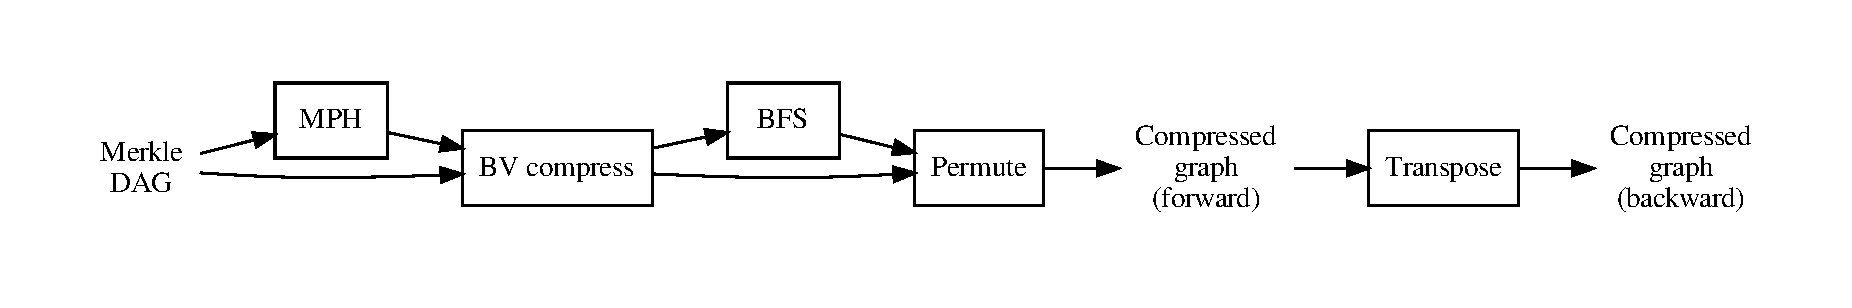
\includegraphics[width=\linewidth,trim=1cm 1cm 1cm 1cm]{img/compression/compression_steps-nofiles}
  \caption{Graph compression pipeline. Individual compression steps are denoted
    with boxes; notable compression input/output artifacts as free text. The
    last transposition step is optional and only needed to visit the graph
    backwards.}%
  \label{fig:compression-pipeline}
\end{figure*}
% TODO: cluster box around the new part of the pipeline

To compress the dataset we use the WebGraph framework to realize the
compression pipeline shown in \cref{fig:compression-pipeline}. The
pipeline input is a simple graph representation (\emph{Merkle DAG} in the
figure) as a pair of textual nodes and edges file. These files use the
``edges'' format described in \cref{sec:edges-format}: the nodes file
consists of one node label per line; the arcs file consists of one
source/destination pair of node labels per linel; each label is a \gls{SWHID}.
Then, the following steps are executed in order:\footnote{we refer to the
WebGraph documentation on how to practically run them:
\url{http://webgraph.di.unimi.it/}}

\paragraph{MPH}
Generate a \emph{\gls{MPH} function}~\cite{GOVFSCF} which maps input
node labels to the set $\{0,\ldots,N-1\}$ consecutive integers, where $N$ is
the number of input nodes. The resulting \gls{MPH} function will be used in the
following to quickly associate \emph{an} integer to node labels without
incurring the risk of collisions.

\paragraph{BV compress}
Compress the adjacency matrix of the graph using gap compression and the other
techniques described in \cref{sec:compression-background}, but without
relying on a sensible ordering of nodes yet. The output of this step is a
\emph{BV graph}~\cite{BoVWFI}.

\paragraph{BFS}
As discussed in \cref{sec:compression-background}, finding a node
ordering that, by permuting rows, maximizes various locality properties on the
graph adjacency matrix is key to achieving good compression. Unlike web
graphs, version control system graphs do not sport ready-to-use ordering
heuristics (such as the URL of each page) that are compression friendly. In
fact, given that native VCS node identifiers are generally based on
cryptographic checksums (e.g., SHA1), the links from one node to the next will
tend to jump \emph{randomly} from one identifier to another in the space of all
possible identifiers.

Experimentally, we have verified that a breadth-first visit of the corpus graph,
starting from graph roots (origin nodes pointing to snapshot nodes in the
graph) and traversing down towards leaves (file contents) achieves good
compression results compared to other orderings.  The \emph{BFS} step of the
compression pipeline thus performs such a visit on the entire BV graph.

\paragraph{Permute}
Once the BFS ordering of nodes is known, this step will reorder nodes (as well
as rows in the compressed adjacency matrix, performing all needed adaptations)
according to BFS order. The result of this step is another compressed graph, in
the same format than the original BV graph but with a better compression ratio.

\paragraph{Transpose}
Strictly speaking, the graph structure of the input dataset can be traversed
only in one direction---from origins roots towards file content leaves. It is
not uncommon for repository mining use cases to need to traverse the graph in
the opposite direction though. For instance, looking up where a given file (or
directory, or commit, etc.) has been found requires such \emph{backward}
visits.

As backward visits correspond to forward visits on the \emph{transposed} input
graph, one can optionally generate a compressed representation of the
transposed input graph and use it in addition (or alternatively) to the
compressed graph obtained thus far. WebGraph supports generating the compressed
representation of the transposed graph directly from the compressed (forward)
graph. If desired, the \emph{Transpose} step in the compression pipeline will
take care of this.

\subsection{Compression results}%
\label{sec:compression-bfs-results}

\begin{table}
  \centering
  \caption{Compression time breakdown}%
  \label{tab:compression-bfs-time}
  \begin{tabular}{l r}
    \multicolumn{1}{c }{\textbf{Step}}
    & \multicolumn{1}{c}{\textbf{Wall time} (hours)} \\
    \hline\hline
    MPH          & 2 \\
    BV Compress  & 84 \\
    BFS          & 19 \\
    Permute      & 18 \\
    Transpose    & 15 \\
    \hline
    \emph{Total} & 138 ($\approx$6 days) \\
  \end{tabular}
\end{table}

Compressing the full corpus is a resource-intensive endeavor. The wall time
breakdown to perform the various steps on the initial dataset is given in
\cref{tab:compression-bfs-time}, totaling less than 6 days of compression
time.

Timings have been taken on a server equipped with 24 CPUs and 750\,GB of
RAM\@. Note however, that such huge amounts of RAM are not actually \emph{needed}
for compression; minimum RAM requirements correspond to the resources needed to
load the final compressed graph in memory. The only step that used more than
100\,GB of RAM was the BFS visit, which used a memory mapping to access the BV
graph on disk using RAM as cache. Recent results on BFS memory
efficiency~\cite{hagerup2019bfs} further confirm that the BFS step is not an
impediment on the general applicability of the approach.

We also stress that even \emph{if} significantly more resources were needed for
compression than for exploitation of the compressed result, that would be an
acceptable trade-off as: (1) compression can be done once and reused many times
(possibly by other research groups), and (2) compression resources can be
rented for one-time use, e.g., on public clouds.

\smallskip

\begin{table}
  \centering
  \caption{Compression results. Compression ratios are w.r.t.~the
    information-theoretical lower bound for graphs with the same density.}%
  \label{tab:compression-bfs-results}

  \hfill
  \begin{tabular}{lr}
    \multicolumn{2}{c}{\textbf{Forward (original) graph}} \\
    \hline\hline
    total size         & 91~GiB \\
    bits per arc       & 4.91 \\
    compression ratio  & 15.8\% \\
    \hline
  \end{tabular}
  \hfill
  \begin{tabular}{lr}
    \multicolumn{2}{c}{\textbf{Backward (transposed) graph}} \\
    \hline\hline
    total size         & 83~GiB \\
    bits per arc       & 4.49  \\
    compression ratio  & 14.4\% \\
    \hline
  \end{tabular}
  \hfill
\end{table}

Compression results are shown in \cref{tab:compression-bfs-results}.
Besides the raw datum of less than 5 bits per arc, which shows that the
compression is very effective in practice, the compression ratio
($\approx$15\%) with respect to the information-theoretical lower bound of
$\log {n\choose m}$ for a graph with $n$ nodes and $m$ arcs is about three
times the one typical for web graphs, which are highly redundant, but
significantly better than the typical values for social networks, which are
above 50\%. Moreover, as it often happens in networks generated by human
activity, the transposed graph shows better compression performance because the
in-degree distribution (shown in \cref{fig:compression-indegree}) has a fatter
tail than the out-degree distribution, (\cref{fig:compression-outdegree})
resulting in nodes with very dense predecessor lists.

\begin{figure}
    \centering
    \begin{subfigure}[b]{.49\textwidth}
        \centering
        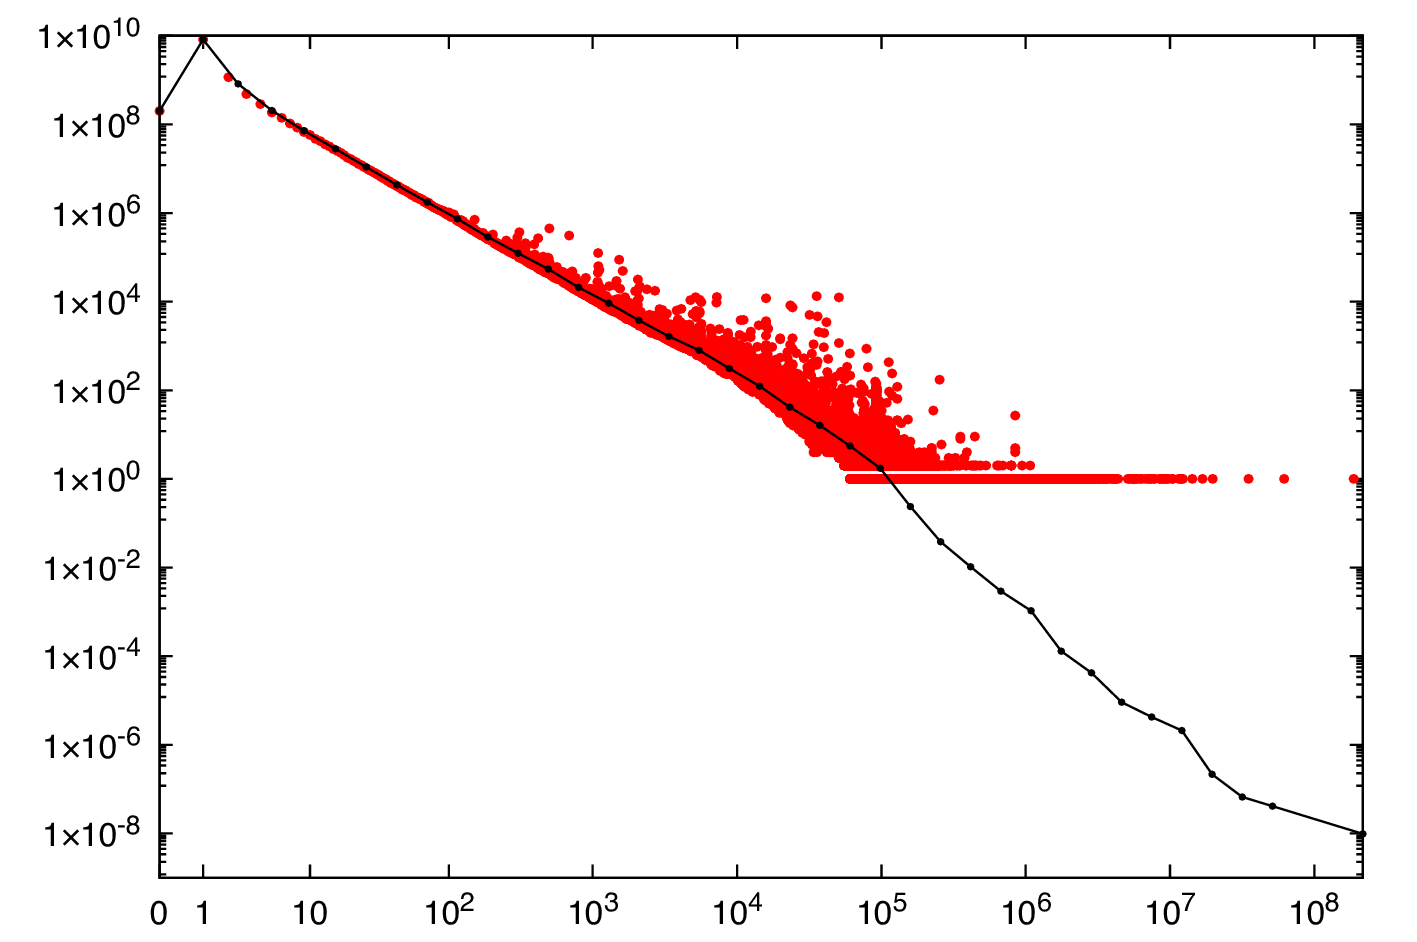
\includegraphics[width=\linewidth]{img/compression/indegree.png}
        \caption{Indegrees.}%
        \label{fig:compression-indegree}
    \end{subfigure}\hfill
    \begin{subfigure}[b]{.49\textwidth}
        \centering
        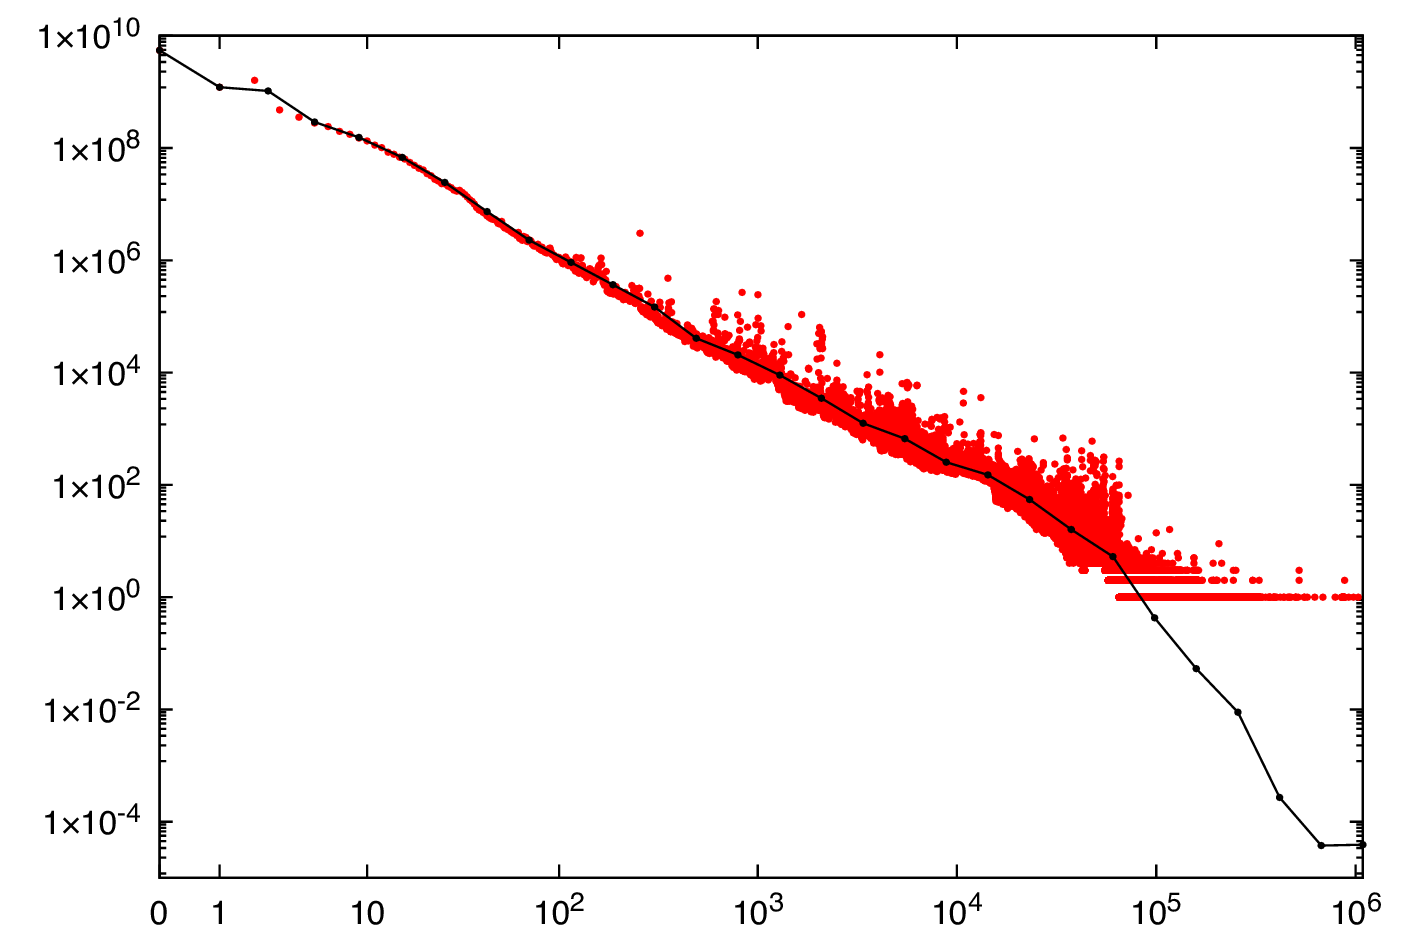
\includegraphics[width=\linewidth]{img/compression/outdegree.png}
        \caption{Outdegrees.}%
        \label{fig:compression-outdegree}
    \end{subfigure}
    \caption{Indegree and oudegree distributions for the entire corpus as a
    graph. Plots show both frequency (red dots) and Fibonacci binning (solid
    black line), which highlight more clearly the shape of the associated
    distribution~\cite{VigFB}. Note how the in-degree distribution has a fatter
    tail than the indeegree one leading, as we will show experimentally, to
    better compression (but worse traversal) performances for the transposed
    graph.}%
    \label{fig:compression-inoutdegree}
\end{figure}

Practically speaking, either direction of the input corpus can be fit in less
than 100\,GB of RAM, even including the 4\,GB type map discussed above. Such an
amount of memory can be easily installed on either powerful workstations or
cheap server-grade hardware---at current market
rates,\footnote{\url{https://jcmit.net/memoryprice.htm}, accessed 2019-10-18}
100\,GB of main memory costs less than 300 U.S.~dollars. Fitting \emph{both}
graph directions on workstation deployments might be more challenging, but it
is not always needed (e.g., one can choose to load only one graph direction
depending on experimental needs) and still fit cheap server-grade deployments
by current standards.

\subsection{Compression with Layered Label Propagation}%
\label{sec:llp-compression}

Further compression improvements can be achieved by the \acrfull{LLP}
algorithm~\cite{BRSLLP} presented in \cref{sec:compression-background}
to reorder nodes. The \gls{LLP} algorithm finds locality-preserving orders by
clustering nodes in close proximity together.  Similar to the \gls{BFS}, this
algorithm is particularly interesting for our use case as it is unsupervised,
and does not rely on prior information on the clusters present in the graph.
The idea behind the clustering algorithm is to randomly distribute communities
to the nodes in the graph, then iteratively assign to each node the community
most represented in its neighbors.

\gls{LLP} is more costly than simple \gls{BFS}-based compression in both time
and memory. Even though the algorithm has a linear time complexity, it does
multiple iterations on the graph and is significantly slower than the \gls{BFS}
which is just one single traversal.  Moreover, keeping track of the communities
requires a total of 33 bytes per node, which increases the RAM requirements to
more than 600\,GiB.

Because of these constraints, it is unrealistic to run the \gls{LLP} algorithm
on the uncompressed version of the graph which already takes around 800\,GiB of
RAM. Thus, instead of replacing \gls{BFS} reordering compression, the \gls{LLP}
reordering is computed \emph{from} the previously compressed graph, and
therefore comes after the full compression pipeline shown in
\cref{sec:compression-pipeline}.

\begin{figure*}
  \centering
  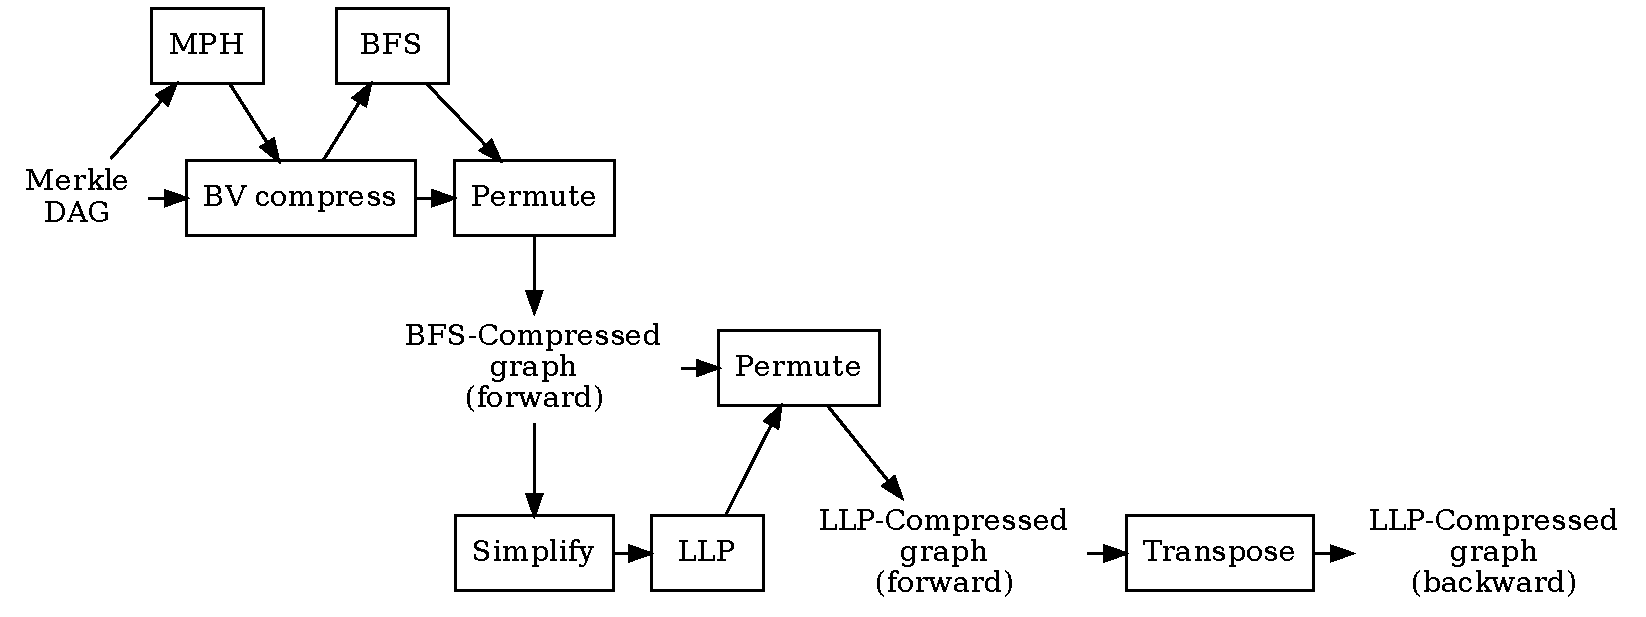
\includegraphics[width=\linewidth]{img/compression/compression_steps_llp}
    \caption{Graph compression pipeline using \gls{LLP} ordering.}%
  \label{fig:llp-compression-pipeline}
\end{figure*}

\Cref{fig:llp-compression-pipeline} shows the full compression pipeline
augmented with \gls{LLP} reordering. Because the algorithm tries to find
clusters of nodes which share a common neighborhood, it operates on the
\emph{undirected} version of the graph, i.e., a graph in which all the edges
are transitive and can be used in both directions. This ``symmetric'' graph can
be obtained by running the \textbf{Simplify} step, which returns a loopless and
symmetric graph from the \gls{BFS}-compressed graph. This symmetric graph is
then fed to the \textbf{LLP} step, which computes the reordering.

The \gls{LLP} algorithm is parametrized by a list of $\gamma$ values, a
``resolution'' parameter which defines the shapes of the clustering it
produces: either small, but denser pieces, or larger, but unavoidably sparser
pieces. The algorithm then combines the different clusterings together to
generate the output reordering. $\gamma$ values are given to the algorithm in
the form $\displaystyle \frac{j}{2^k}$; the default $\gamma$ values used in the
\gls{LLP} implementation of the WebGraph framework are:

\[
    \Bigl\{
    1,~\frac{1}{2},~\frac{1}{4},~\frac{1}{8},~\frac{1}{16},~\frac{1}{32},~%
    \frac{1}{64},~\frac{1}{128},~\frac{1}{256},~\frac{1}{512},~\frac{1}{1024},~0
    \Bigr\}
\]

However, the combination procedure is very slow, and giving that many $\gamma$
values could take several months in our case. We thus need to narrow down a
smaller set of values that give good compression results.
In order to find an
optimal combination of $\gamma$ values for compressing the graph of software
development, we performed a hyperparameter sweep with different lists of
values. The results are shown in \cref{tab:compression-llp-gammas}.

\begin{table}
  \centering
  \caption{LLP compression results for different $\gamma$ values, compared to
    the BFS-compressed baseline.}%
  \label{tab:compression-llp-gammas}

      % \setlength\extrarowheight{1em}
  \renewcommand{\arraystretch}{1.5}
  \begin{tabular}{l r r r r r r}
      \hline \textbf{$\gamma$ values} \hspace{4em}
      & \multicolumn{3}{c}{\textbf{Forward graph}}
      & \multicolumn{3}{c}{\textbf{Transposed graph}} \\

      % \hline
      & size & bits/arc & ratio
      & size & bits/arc & ratio \\

      \hline \emph{BFS baseline}
      & 118\,GiB & 5.2 & 16\%
      & 94\,GiB & 4.11 & 13\% \\

      \hline $0$, $1$, $\frac{1}{64}$
      & 91\,GiB & 3.98 & 12\%
      & 82\,GiB & 3.58 & 11\% \\

      \hline $\frac{1}{2}, \frac{1}{4}, \frac{1}{8}, \frac{1}{16}$
      & 77\,GiB & 3.37 & 11\%
      & 62\,GiB & 2.71 & 8\% \\
    \hline
  \end{tabular}
\end{table}

As can be seen, the compression ratio is significantly improved using the LLP
algorithm. In the best case, the size of the compressed graph is reduced by
35\% from the BFS baseline. If the graph is to be loaded in fully RAM, such
differences are very significant to determine the practicality of the approach
on some given hardware. The additional complexity of adding LLP in the
compression pipeline can therefore be easily justified.

An interesting result is that smaller values of $\gamma$ seem to generate
better compression ratios.
The effect of a given $\gamma$ is that the density of the sparsest cluster is
at least $\frac{\gamma}{\gamma+1}$, so large $\gamma$ values imply small, more
dense clusters.  It is reasonable to assume that since the graph is very sparse
to start with, such clusters are not that useful.

\bigskip

The main takeaway of this section is that, from a size perspective, graph
compression \emph{can be used} to fit the structure of immense VCS datasets in
memory on a single machine with limited hardware resources. Using a simple
graph traversal for reordering, the graph size can be brought down to under
around 150 GiB. Depending on the resources available for compression, the
graph can be further compressed by applying more expensive reordering
algorithms like \gls{LLP}.


\section{Exploitation}%
\label{sec:compression-exploitation}

We now move to the speed perspective to experimentally assess how effectively
the obtained compressed representation of ultra-large-scale repository
collections can be leveraged to perform repository mining experiments. We first
perform a few domain-agnostic benchmarks (e.g., graph visits, arc traversal
time) and then perform a domain-specific experiment.


\subsection{Graph traversal}%
\label{sec:compression-exptraversal}

In the worst case of any given mining experiment, one will have to traverse the
entire corpus to obtain some insights. Hence it is important to know the
baseline of how long a single traversal takes.
\Cref{tab:compression-bfs-benchmark} shows the results of benchmarking complete
graph visits in breadth-first order (BFS), with no parallelism (single thread)
for both the original and transposed graphs. Timings have been measured on a
server equipped with 3\,GHz Intel Xeon Gold 6154 CPUs (only one of which has
been used for the visits), with enough RAM to load either graph direction in
memory without swapping to disk.

Results show that the in-memory approach delivers impressive performances. A
full visit of the forward graph takes less than 2 hours with a throughput
nearing 2 million nodes per second, or about 500 nanoseconds per node. Visiting
the transposed graph is slower due to the already discussed differences in
in-degree vs.\ out-degree distributions, but still very fast in absolute terms:
the full transposed graph can be visited in little more than 3 hours with a
throughput nearing 1 million nodes/second (1 $\mu$s/node).

\Cref{tab:compression-arc-benchmark} shows the results of benchmarking
random access to nodes and edges in the graph. A random sample of 1 billion
nodes (8.3\% of the entire graph) has been taken, enumerating for every node
all of its successors.  Results show that having the graph in memory gives
impressive results also in terms of random lookup time, with minimal overhead
due to the compressed representation. On the original graph, looking up the
successor of a node takes 83 nanoseconds on average, close to the 50--60\,ns
estimates for current DRAM random access memory. Arc lookup on the transposed
graph is slower, as already observed for full graph visits.

\begin{table}
  \centering
  \caption{Full graph visit benchmarks for a single-threaded BFS visit}%
  \label{tab:compression-bfs-benchmark}
  % \begin{tabular}{lr}
  %   visit order    & BFS \\
  %   concurrency    & single thread \\
  %   visited nodes  & \num{11683687950} (entire graph) \\[2ex]
  % \end{tabular}
  
  \hfill
  \begin{tabular}{lr}
    \multicolumn{2}{c}{\textbf{Forward (original) graph}} \\
    \hline\hline
    wall time      & 1h48m \\
    throughput     & 1.81\,M nodes/s \\
                   & (553\,ns/node) \\
    \hline
  \end{tabular}
  \hfill
  \begin{tabular}{lr}
    \multicolumn{2}{c}{\textbf{Backward (transposed) graph}} \\
    \hline\hline
    wall time      & 3h17m\\
    throughput     & 988\,M nodes/s \\
                   & (1.01\,$\mu$s/node) \\
    \hline
  \end{tabular}
  \hfill
\end{table}

\begin{table}
  \centering
  \caption{Arc lookup benchmarks for 1 billion random nodes}
  \label{tab:compression-arc-benchmark}

  % \begin{tabular}{lr}
  %   sample size   & 1 B nodes (8.3\% of entire graph)
  % \end{tabular}
  % \\[2ex]

  \hfill
  \begin{tabular}{lr}
    \multicolumn{2}{c}{\textbf{Forward (original) graph}} \\
    \hline\hline
    visited arcs  & \num{13644656586} \\
    throughput    & \num{12018223}\,arcs/s \\
                  & (83\,ns/arc) \\
    \hline
  \end{tabular}
  \hfill
  \begin{tabular}{lr}
    \multicolumn{2}{c}{\textbf{Backward (transposed) graph}} \\
    \hline\hline
    visited arcs  & \num{13625228259} \\
    throughput    & \num{9453613}\,arcs/s \\
                  & (106\,ns/arc) \\
    \hline
  \end{tabular}
  \hfill
\end{table}



\subsection{Source code artifact multiplication}%
\label{sec:compression-expmultiplication}

As the goal is to benchmark the potential of the proposed approach for
ultra-large-scale repository analysis, we focus on a domain-specific experiment
which needs to intensely crawl VCS histories in the studied corpus.
Specifically, we will replicate the experiments of~\cite{swh-provenance-emse} to
quantitatively assess the \emph{multiplication factor} of source code artifacts
in the corpus. We will measure:
\begin{enumerate}

\item The multiplication of source code file contents across commits
  (\emph{blob $\to$ revision multiplication} in the following), i.e., how much
  the same unmodified file content reappears in different commits, regardless
  of which origins they were found in. This measure correlates with and
  is a requirement for Type 1 (exact) clone
  detection~\cite{bellon2007comparison}, both within and across repositories.

\item The multiplication of commits across origins (\emph{revision $\to$ origin
  multiplication}), i.e., the frequency with which the same commit reappears
  in different repositories. The fact that the same commit reappears at
  different origins is partly the result of collaborative social coding,
  but can also hint at the migration of development from one platform to
  another.

\end{enumerate}

In the given data model, blob $\to$ revision multiplication can be measured by
iterating on all nodes of type ``blob'', then performing a visit on the
transposed graph that only follows arcs leading to revision nodes---i.e.,
excluding (the transposed of) arcs snapshot $\to$ revision, release $\to$
revision, and origin $\to$ snapshot---and finally counting the number of
revision leaves reached with the visit. Results can then be visualized as a
distribution of the ``popularity'' of blobs across commits.

Note that, even if the compressed graph representation does not natively store
type information for arcs, we can use the type map discussed in
\cref{sec:compression-comp-scope} to stop the visit when it is no longer
possible to reach additional revision nodes.

The approach for determining revision $\to$ origin multiplication is similar.
The only difference is that visits will start from commit nodes and stop at
origin nodes (graph roots), which can then be counted and visualized as before.

The chosen approaches are naive from an algorithmic point of view---the same
edges will be traversed repeatedly for different input nodes,
resulting in a time complexity of $O(V\cdot E)$, which is generally considered
impractical on graphs of this scale.  Having already established the overall
efficiency of full graph visits, we chose these approaches for the sake of
simplicity and explainability.

More time-efficient approaches are possible and would be equally well supported
by the compressed graph framework. For instance, one could propagate ancestry
information during the visit, obtaining linear-time algorithms at the price of
extra memory requirements (or extra memory mapping). Our main point is that the
entire corpus \emph{itself} can be fit in relatively little memory and accessed
with excellent performances; other algorithmic considerations will vary
according to the needs of the planned mining task, as they always do.


\subsection{Results}

\Cref{fig:compression-distrib-cnt-rev} shows the multiplication factor
distribution for blob $\to$ revision, measured on a random sample of 953\,M
blobs. Looking at the cumulative distribution (top line) the average
multiplication factor appears to be very high. There are more than 100 million
blobs ($\approx$20\% of the sample) that are duplicated more than one
thousand times in different commits; 10 million blobs (1\%) reoccur in more
than ten thousand commits; and 1 million blobs (0.1\%) in more than a
hundred thousand commits.

As we did not partition by origin, these results do not say whether this
multiplication is due to the long life of unmodified source code files in
long-lived code bases, or instead due to reuse of the same unmodified files
across different repositories. It would be easy to modify the experiment to
follow edges up to origin nodes to determine that.

\smallskip

\begin{figure}
  \centering
  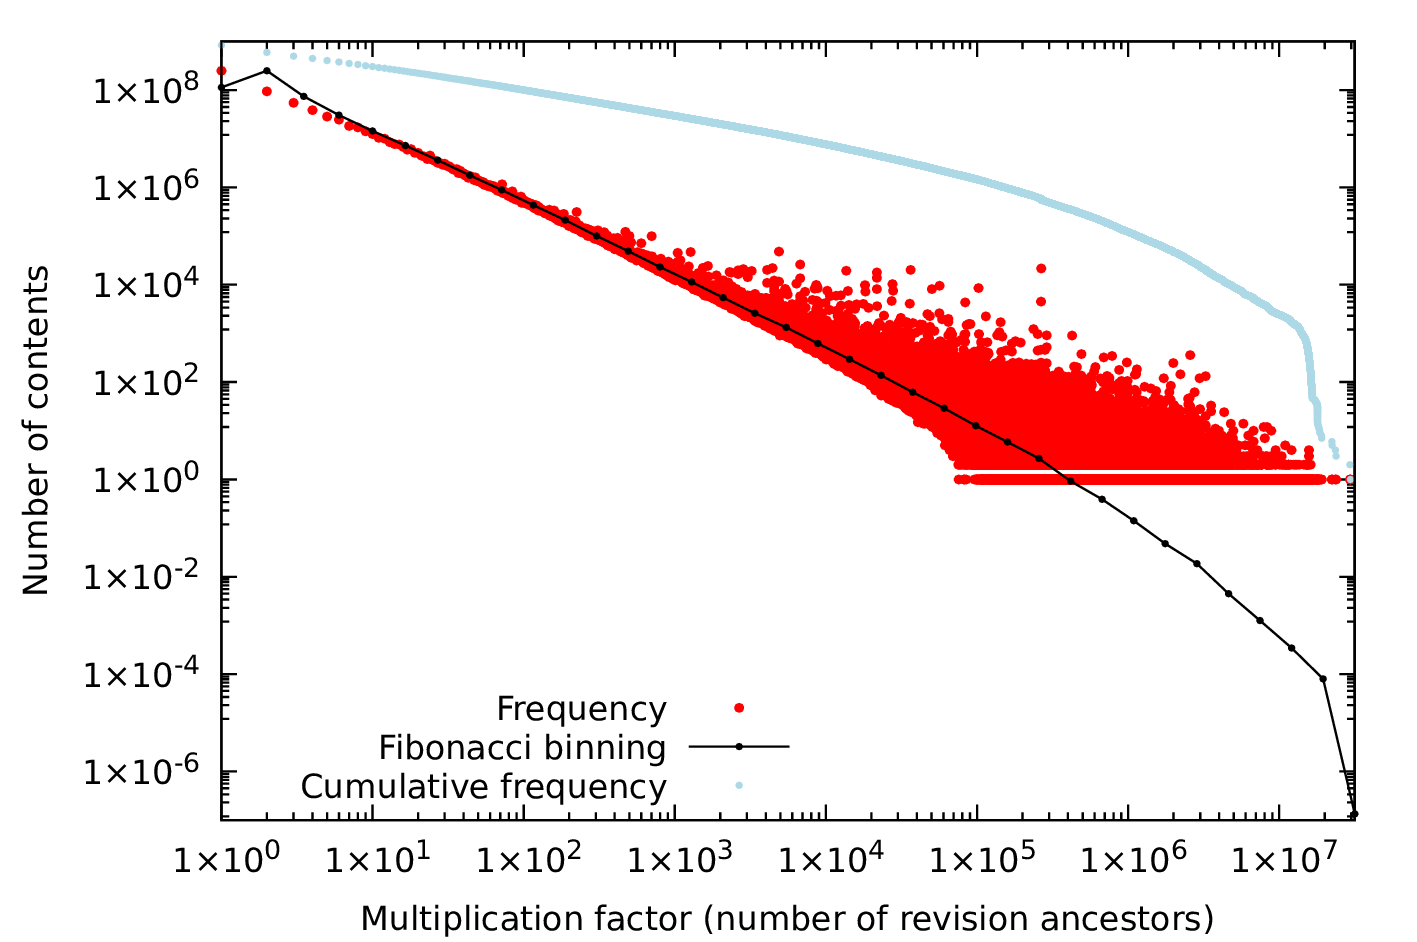
\includegraphics[width=0.7\linewidth]{img/compression/distributions/contents.png}
  \caption{Content $\to$ revision multiplication, i.e., how often file contents
    (Y axis) reoccur unmodified in different commits (X axis), based on a
    random sample of 953\,M blobs (17\% of all blobs).}%
  \label{fig:compression-distrib-cnt-rev}
\end{figure}

\begin{figure}
  \centering
  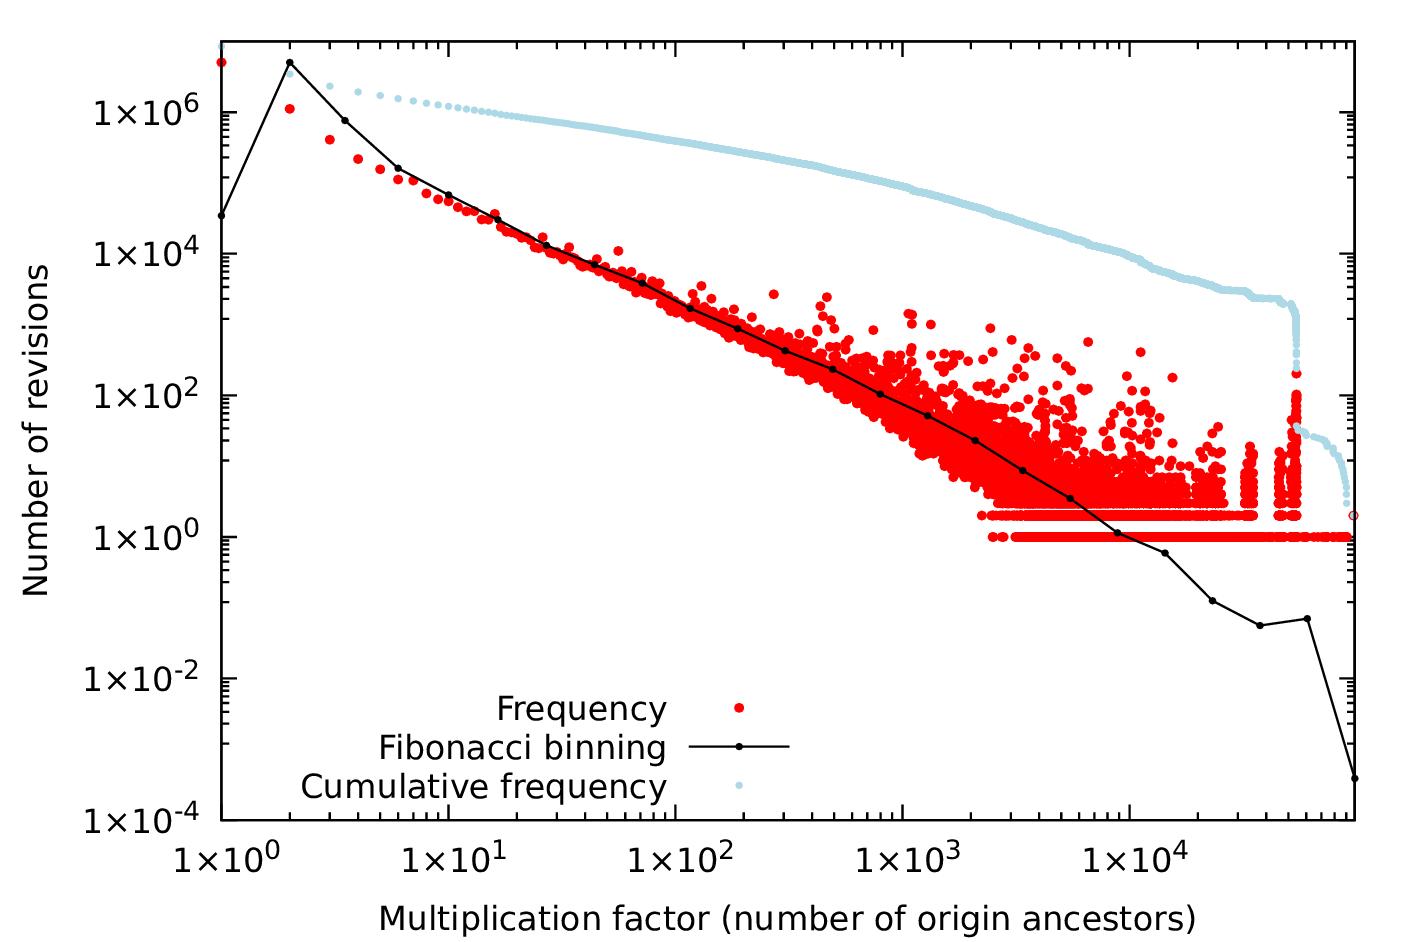
\includegraphics[width=0.7\linewidth]{img/compression/distributions/revisions.png}
  \caption{Revision $\to$ origin multiplication, i.e., how often commits (Y
  axis) reoccur in different repositories (X axis), based on a random sample of
  8.5\,M revision (0.77\% of all revisions).}%
  \label{fig:compression-distrib-rev-ori}
\end{figure}

\Cref{fig:compression-distrib-rev-ori} shows analogous results for the
revision $\to$ origin layer, on a random sample of 8.5\,M revisions. To interpret
them, it is important to realize how it happens that the same commit (i.e.,
with an identical SHA1 identifier) is found in different repositories. The main
reason is the distributed nature of modern version control systems, whose
repositories are massively represented in the corpus under analysis. Developers
that work together using Git will have individual repositories that communicate
by exchanging SHA1-identical commits. Furthermore the pull request development
model~\cite{gousios2014pullrequests} popularized by GitHub natively creates new
repositories (hosted at different origin URLs) that initially contains all
commits (unmodified) of the originally ``forked'' repository.

The cumulative distribution of \cref{fig:compression-distrib-rev-ori} measures
the amount of redistribution of the same commits via different repositories in
our corpus. 5 million commits (60\% of the sample) can be found in a single
repository only, but multiplication grows quickly from there: 100 thousand
commits (1\%) can be found in 1000 repositories or more and 10 thousand commits
(0.01\%) can be found in 10 thousand repositories or more. We observe that
software development is nowadays very distributed, to a point of strong
resiliency to the disappearance of a single point of source code distribution.

\begin{figure}
  \centering
  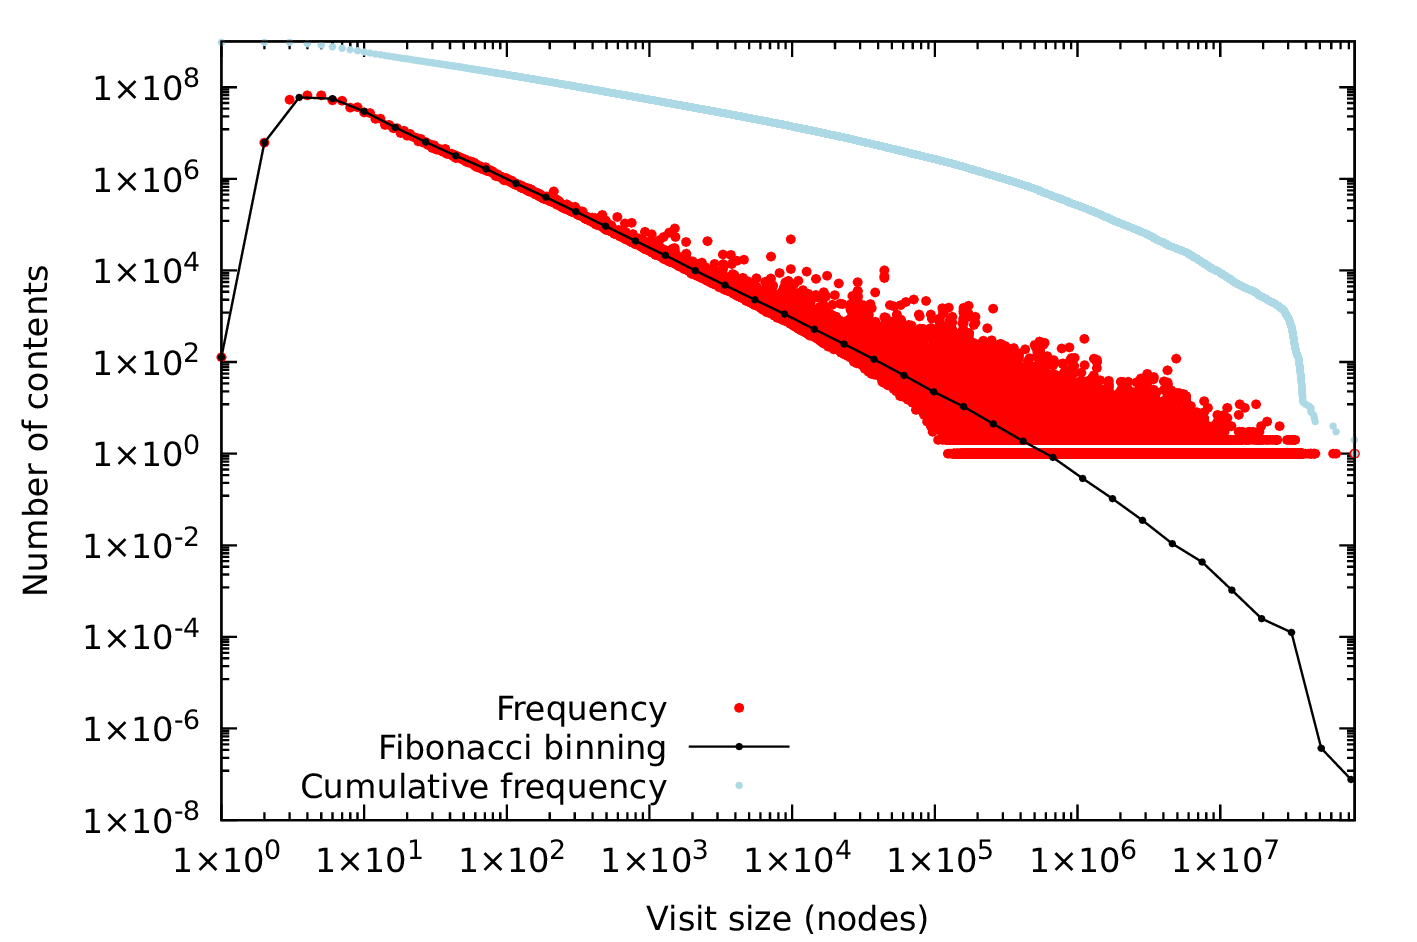
\includegraphics[width=0.7\linewidth]{img/compression/distributions/contents_node_size.png}
  \caption{Visit size, as the number of visited nodes, for measuring
    blobs $\to$ revision multiplication on the same sample of
    \cref{fig:compression-distrib-cnt-rev}.}%
  \label{fig:compression-size-cnt-rev}
\end{figure}

\begin{figure}
  \centering
  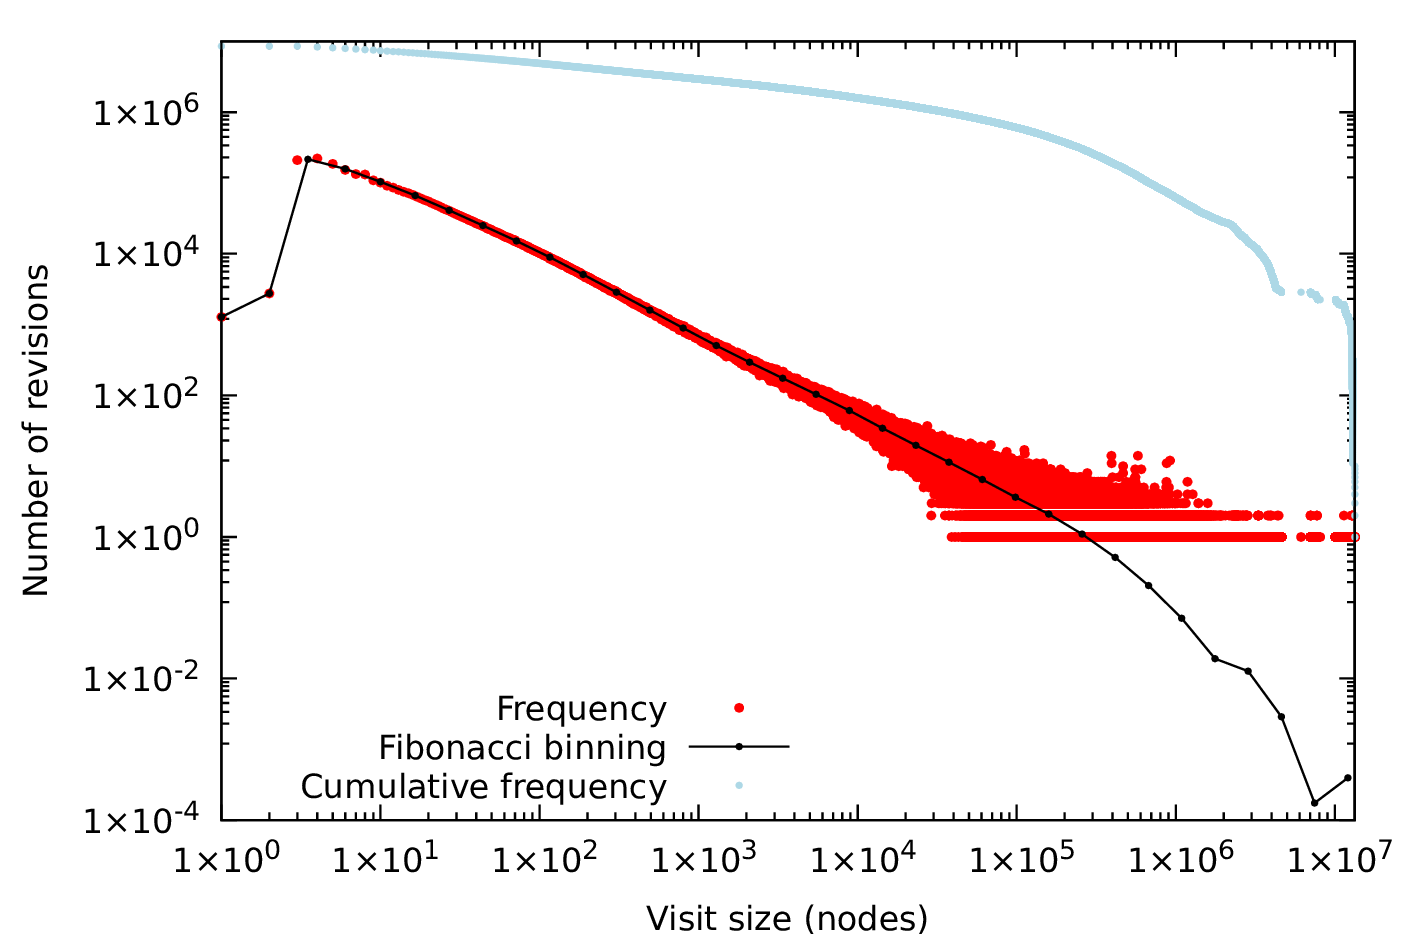
\includegraphics[width=0.7\linewidth]{img/compression/distributions/revisions_node_size.png}
  \caption{Visit size, as the number of visited nodes, for measuring
    revision $\to$ origin multiplication on the same sample of
    \cref{fig:compression-distrib-rev-ori}.}%
  \label{fig:compression-size-rev-ori}
\end{figure}

\smallskip

To better appreciate the graph-intensive nature of realizing the above two
experiments in practice, we have also measured visit sizes.
\cref{fig:compression-size-cnt-rev} and \cref{fig:compression-size-rev-ori}
show the results in terms of visited nodes.

Content $\to$ revision visits traverse significantly more nodes (and edges)
than revision $\to$ origin visits. This is expected due to the respective sizes
of the traversed subgraphs and it is a dominant factor over the fact that, on
average, the filesystem layer of the graph (blobs $\cup$ directory nodes) has
shorter graph paths than the revision layer (VCS repositories of large software
projects such as the Linux kernel can have commit chains nearing 1\,M commits
in length).

\smallskip

In terms of timings, the presented results have been obtained on multi-core
machines with, respectively, 20 $\times$ 2.40\,GHz CPUs (for
blob $\to$ revision) and 36 $\times$ 3.00\,GHz CPUs (for revision $\to$ origin),
letting the experiments run for about 2.5 days in total. In spite of the naive
$O(V\cdot E)$ algorithmic approaches chosen, such short running times have
allowed to process very large subgraphs.

\smallskip

The main conclusions we can draw from these experiments are that: (1) graphs
are suitable data models for conducting version control system analyses,
including code duplication experiments; and (2) \emph{compressed} graphs allow
such analyses to be performed at ultra-large-scale with impressive graph
traversal performances.

\section{Discussion}%
\label{sec:compression-discussion}

Both size-wise and performance-wise the results of applying graph compression
to VCS graphs to support their ultra-large-scale analysis appear to be more
than satisfactory. VCS graphs compress well both in absolute terms and in
comparison with other large graphs compressed in the past (e.g., web graphs).
Graph visit performances are consistent with main memory access time and can
support visit-intense VCS analysis needs well on limited resources.
%
That notwithstanding we are not claiming that graph compression is a silver
bullet for VCS analysis. We discuss in this section limitations and trade-offs
that apply to the proposed approach.


\subsection{Graph design}

As mentioned in \cref{sec:compression-comp-scope} there exists a clear
\emph{space/time trade-off} between what fits in main memory and what should be
left in secondary storage. Our choice---graph structure + node types in memory,
everything else in secondary storage---will enable speeding up many use cases,
under the assumption that VCS traversal is a common performance bottleneck of
large-scale analyses.

Other choices are possible, valid, and can still be supported by graph
compression, allowing \emph{more} information to fit in RAM than what would be
possible otherwise. We discuss a few possible scenarios below.

One might decorate graph nodes with \emph{additional metadata} to be used
during traversals and should hence be looked up efficiently. For instance,
commit nodes might be equipped with in-RAM timestamps (either absolute, or
relative, as in logical clocks) to direct visits to choose the earliest
occurrence of what is being sought.
Graph compression will be useful nonetheless, and the induced re-labeling of
nodes to integers often enables storing additional metadata in memory in very
compact ways, as we did for the type map.  Attaching metadata to graph
\emph{arcs} is more tricky, but limited support for doing so is offered by
WebGraph\footnote{via the \texttt{webgraph.labelling} package} and other
state-of-the-art frameworks. This is further discussed in
\cref{chp:graph-metadata}.

\emph{Graph semantics} is another variable that can be played with. In the
presented case study graph leaves are unmodified file contents, enabling the
tracking of bit-identical clones. One might instead use checksums of
\emph{normalized} source code files (e.g., removing spaces), obtaining the
canonical definition of Type 1 clones, or parse source code files to ASTs and
associate intrinsic identifiers to them (for Type 2 clones).

\emph{Graph granularity} can also be increased, e.g., by adding nodes
corresponding to individual lines of codes (normalized or otherwise). Doing so
would enable tracking SLOC cloning and migrations at an unprecedented scale. It
will also significantly increase the graph size, by a factor close to the
average length of source code files (in SLOCs). The resulting graph will be
huge, but as graph compression techniques are used in production on web graphs
(with nodes in the trillions), we are confident they can scale up to SLOC
analysis needs.


\subsection{Limitations}%
\label{sec:compression-limitations}

A limitation of using static graph compression over classic information systems
to store the data to be analyzed is that \emph{compression is not incremental}
with regards to the arrival of new artifacts (commits, files, etc.), due to the
need of reordering nodes and updating the compressed representations of
adjacency lists. Considering that popular VCS repositories receive hundreds of
new commits a day, the already mentioned exponential growth of original
publicly available code, and the observed multi-day compression times---this
means that analyzed data will be chronically out-of-date w.r.t.~reality.

This limitation is not problematic for research use cases, where datasets are
generally frozen before conducting an experiment; but it might be problematic
for other needs, like live-monitoring of interconnected private/public code
bases. This is not a novel problem for other fields in which graph compression
is applied, such as web search and social network analysis. Some compression
techniques (e.g., $k^2$-trees~\cite{brisaboa2017compressed}) lend themselves
more or less naturally to be adapted to the dynamic case, but with a definite
degradation in compression performances. A common mitigation technique that can
be applied to all static compressors is to use dynamic, updatable \emph{overlay
  graphs} on top of the compressed one. Overlays will be more memory-hungry,
but they are ephemeral: periodically the underlying compressed graphs will be
recompressed to regain storage-efficiency.

It is also theoretically possible to exploit knowledge of the graph topology to
leave ``gaps'' in the node ordering that can be used as room for adding new
nodes of a given type dynamically to the compressed graph representation. We
intend to explore this possibility in future work.

\section{Related work}%
\label{sec:compression-related}

\subsection{Large-scale mining approaches}

Other large-scale repository mining approaches have been proposed in the past.
%
Boa~\cite{dyer2013boa} has pioneered the idea of a mutualized infrastructure
hosting both data and compute resources to perform large-scale analyses on
source code artifacts such as those discussed in this chapter. Our notion of
``ultra-large-scale'' is different, with a case study 100x larger by several
metrics (projects, files, commits, etc.). The compute approach is also
different, with Boa relying on distributed clusters (Hadoop) and our approach
relying on a single machine. Direct performance comparisons are not possible as
we have not replicated their experiments, but our results hint at a very
significant speedup when the main bottleneck is history traversal. It would be
interesting---and it seems entirely possible---to realize an infrastructure
like Boa, based on a compressed VCS representation like the one proposed in
this chapter.

World of Code (WoC)~\cite{mockus2019woc} is a recent attempt at a mutualized
infrastructure for large-scale VCS analyses. While limited to GitHub---contrary
to our case study that also encompasses GitLab and major package
repositories---the target scale of WoC is similar to ours. The compute approach
is different, with WoC relying on distributed databases running and ours on a
single machine. The advantage of WoC is that it maintains pre-computed
mappings, e.g., from files and directories to the places they come from,
choosing a different spot than ours in the classic space/time trade-off. The
approach proposed here looks more appealing in terms of cost and ease of
deployment. But the two approaches are complementary: WoC might benefit from an
\emph{additional} compressed graph representation that would shine when users
need to explore on the fly (and as quickly as possible) artifact relationships
that are not available as pre-computed mappings.

Large-scale VCS analyses have been conducted in the past, usually at much
smaller scale than ours. An exception is~\cite{swh-provenance-emse}, which
developed a compressed representation for software provenance tracking and used
it to conduct the multiplication experiments that we have replicated in
\cref{sec:compression-expmultiplication}. Both approaches can be applied
to conduct analyses on commodity hardware, but the compression trade-offs are
different: specialized, lossy, and incremental in~\cite{swh-provenance-emse};
general purpose, lossless, but not incremental here.

LISA~\cite{alexandru2019redundancy} is a framework for reducing artifact
redundancy when analyzing VCS-stored source code. It is more fine-grained than
our case study, reaching down to abstract syntax tree nodes. As such it could
deduplicate more, but at the price of requiring a proper parser, which is not
always available and might fail on syntactically incorrect files that one might
still want to analyze. Also, we deal with all kinds of VCS artifacts while LISA
is specific to source code files.

Large-scale experiments on development activities \emph{not} captured by VCS
histories (e.g., pull requests, code reviews, bug tracking, etc.) have also
been conducted. They generally rely on dedicated activity databases, such as
GHTorrent or GitHub Archive~\cite{GHTorrent, ray2014large}. Differences from
the proposed approach are significant both in terms of scope (we focus on VCS
histories, them on other activities) and needed resources.


\subsection{Graph compression techniques}%
\label{sec:graph-compression-techniques}

The problem of finding compression-friendly node orderings was studied from a
theoretical viewpoint in~\cite{CKLCSN}, where the authors show that the problem
of determining the optimal renumbering of nodes is NP-hard, but propose a
heuristic (called ``shingle ordering'') for the problem, based on a fingerprint
of the out-neighborhoods.

More recently,~\cite{DKKCGIRGB} extended the theoretical model of~\cite{CKLCSN}
and designed a novel ordering technique, called \emph{recursive graph
bisection}, that yields the most competitive compression ratios in several
cases. The core idea is to recursively divide the graph in two clusters of the
same size so as to minimize an objective function that estimates the
compressibility of the overall graph when nodes in the first cluster have
smaller identifiers than nodes in the second cluster.

To the best of our knowledge, the first technique would not scale to our use
case. Recursive bisection might have some margin of benefit over a BFS or LLP
reordering, but at the price of a significantly slower computation. We plan to
study this problem in the future.

A complementary approach to storing adjacency lists is that of
$k^2$-trees~\cite{Brisaboa2014152}. In this case, one aims at compactly
representing the adjacency \emph{matrix} of the graph (as opposed to its
adjacency \emph{lists}), exploiting its sparseness.  However, $k^2$-trees do
not scale beyond a few dozen million vertices. They are hence inapplicable to
the target scale of this thesis.

Since successor lists are increasing integers, one can use \emph{succinct data
  structures}~\cite{NavCDS} to store them. A succinct data structure does not
\emph{compress} data, it represents it using the minimum possible number of
bits instead.
More precisely, if an object requires $z$ bits to be represented, a succinct
data structure uses $z+o(z)$ bits.

A simple, practical data structure of this kind is the \emph{Elias-Fano
representation of monotone sequences}~\cite{EliESRCASF}, which are technically
not fully succinct but \emph{quasi-succinct}.
An advantage of the
Elias-Fano representation is the possibility of finding in constant time both
the $k$-th successor and the first successor greater than or equal a
given bound $b$. In particular, the last property makes it possible to verify
adjacency in constant time, and neighborhood intersections in sublinear time.

\emph{Partitioned Elias-Fano}~\cite{OtVPEFI} is a improvement over the basic
Elias-Fano representation: given a number $k$ of parts, an algorithm splits
the successor lists in $k$ blocks in such a way that the space used is
minimized. In this way, dense blocks as those generated by similarity can be
compressed efficiently, with a constant additional cost for the access
operations.

We remark that using a separate succinct encoding for each successor list can
be more efficient than succinctly encoding the entire graph (for example, using
an Elias-Fano list to represent the positions of the ones in the adjacency
matrix, or using truly succinct representations~\cite{FaMSEAG}). This happens
because by Jensen's inequality the average cost \emph{per successor} is
necessarily lower.  However, if one takes also into account the constant costs
associated to storing each successor list, there is a trade-off that has to be
evaluated on a case-by-case basis.  The Elias-Fano representation has been
recently made dynamic~\cite{PiVDEFR} when the universe is polynomial in the
list size, which makes it possible to use it in the case of dynamic graph
representation.

Succinct approaches are particularly useful when the graph has no evident
structure (as in that case reference compression does not really help) and when
reordering the nodes is not possible (as the compression obtained is agnostic
with respect to the distribution of gaps and to similarity). We therefore did
not consider these approaches relevant to the case at hand.
